% Options for packages loaded elsewhere
\PassOptionsToPackage{unicode}{hyperref}
\PassOptionsToPackage{hyphens}{url}
%
\documentclass[
]{book}
\usepackage{amsmath,amssymb}
\usepackage{iftex}
\ifPDFTeX
  \usepackage[T1]{fontenc}
  \usepackage[utf8]{inputenc}
  \usepackage{textcomp} % provide euro and other symbols
\else % if luatex or xetex
  \usepackage{unicode-math} % this also loads fontspec
  \defaultfontfeatures{Scale=MatchLowercase}
  \defaultfontfeatures[\rmfamily]{Ligatures=TeX,Scale=1}
\fi
\usepackage{lmodern}
\ifPDFTeX\else
  % xetex/luatex font selection
\fi
% Use upquote if available, for straight quotes in verbatim environments
\IfFileExists{upquote.sty}{\usepackage{upquote}}{}
\IfFileExists{microtype.sty}{% use microtype if available
  \usepackage[]{microtype}
  \UseMicrotypeSet[protrusion]{basicmath} % disable protrusion for tt fonts
}{}
\makeatletter
\@ifundefined{KOMAClassName}{% if non-KOMA class
  \IfFileExists{parskip.sty}{%
    \usepackage{parskip}
  }{% else
    \setlength{\parindent}{0pt}
    \setlength{\parskip}{6pt plus 2pt minus 1pt}}
}{% if KOMA class
  \KOMAoptions{parskip=half}}
\makeatother
\usepackage{xcolor}
\usepackage{longtable,booktabs,array}
\usepackage{calc} % for calculating minipage widths
% Correct order of tables after \paragraph or \subparagraph
\usepackage{etoolbox}
\makeatletter
\patchcmd\longtable{\par}{\if@noskipsec\mbox{}\fi\par}{}{}
\makeatother
% Allow footnotes in longtable head/foot
\IfFileExists{footnotehyper.sty}{\usepackage{footnotehyper}}{\usepackage{footnote}}
\makesavenoteenv{longtable}
\usepackage{graphicx}
\makeatletter
\def\maxwidth{\ifdim\Gin@nat@width>\linewidth\linewidth\else\Gin@nat@width\fi}
\def\maxheight{\ifdim\Gin@nat@height>\textheight\textheight\else\Gin@nat@height\fi}
\makeatother
% Scale images if necessary, so that they will not overflow the page
% margins by default, and it is still possible to overwrite the defaults
% using explicit options in \includegraphics[width, height, ...]{}
\setkeys{Gin}{width=\maxwidth,height=\maxheight,keepaspectratio}
% Set default figure placement to htbp
\makeatletter
\def\fps@figure{htbp}
\makeatother
\setlength{\emergencystretch}{3em} % prevent overfull lines
\providecommand{\tightlist}{%
  \setlength{\itemsep}{0pt}\setlength{\parskip}{0pt}}
\setcounter{secnumdepth}{5}
\usepackage{booktabs}
\usepackage{amsthm}
\usepackage[ngerman,provide=*]{babel}

% Redefine names for various elements
\renewcommand{\figurename}{Abbildung}
\renewcommand{\tablename}{Tabelle}
\renewcommand{\contentsname}{Inhaltsverzeichnis}
\renewcommand{\partname}{Teil}
\renewcommand{\chaptername}{Kapitel}
\renewcommand{\appendixname}{Anhang}

% The \equationname is not a standard LaTeX command, so we'll define it
\newcommand{\equationname}{Gleichung}

% Define theorem-like environments
\newtheorem{theorem}{Theorem}
\newtheorem{lemma}{Lemma}
\newtheorem{proposition}{Proposition}
\newtheorem{conjecture}{Vermutung}
\newtheorem{definition}{Definition}
\newtheorem{example}{Beispiel}
\newtheorem{exercise}{Übung}
\newtheorem{hypothesis}{Hypothese}

% Redefine proof name
\renewcommand{\proofname}{Beweis}

% Define custom environments
\newenvironment{remark}{\par\textbf{Hinweis.} }{\par}
\newenvironment{solution}{\par\textbf{Lösung.} }{\par}

% Ensure German captions are used
\addto\captionsgerman{
  \renewcommand{\partname}{Teil}
  \renewcommand{\chaptername}{Kapitel}
}

\usepackage{amsthm}
\ifLuaTeX
  \usepackage{selnolig}  % disable illegal ligatures
\fi
\usepackage[]{natbib}
\bibliographystyle{apalike}
\usepackage{bookmark}
\IfFileExists{xurl.sty}{\usepackage{xurl}}{} % add URL line breaks if available
\urlstyle{same}
\hypersetup{
  pdftitle={Statistik 1},
  pdfauthor={Daniel J. F. Gerber},
  hidelinks,
  pdfcreator={LaTeX via pandoc}}

\title{Statistik 1}
\author{Daniel J. F. Gerber}
\date{2024-10-04}

\begin{document}
\maketitle

{
\setcounter{tocdepth}{1}
\tableofcontents
}
\chapter*{Vorwort}\label{vorwort}
\addcontentsline{toc}{chapter}{Vorwort}

Dieses Buch ist im Rahmen meiner Lehrtätigkeit an der FHNW entstanden und frei verfügbar.

\chapter{Einleitung}\label{einleitung}

\section{Worum geht es?}\label{worum-geht-es}

\section{Inhaltlicher Aufbau}\label{inhaltlicher-aufbau}

Dieses Buch umfasst die untenstehenden Inhalte. Die Inhalte wurden hier nach Zwecken sortiert angeordnet:

Stichprobe beschreiben (\textbf{deskriptive Statistik}):

\begin{itemize}
\tightlist
\item
  Arithmetisches Mittel
\item
  Median
\item
  Quantile
\item
  Anteil
\item
  Odds Ratio
\item
  Relatives Risiko
\end{itemize}

Population beschreiben (\textbf{Wahrscheinlichkeitslehre}):

\begin{itemize}
\tightlist
\item
  Zufallsvariable
\item
  Erwartungswert
\item
  Standardabweichung
\item
  Varianz
\item
  Wahrscheinlichkeitsdichte
\item
  Wahrscheinlichkeitsverteilung
\item
  Verteilungen
\end{itemize}

Populationsparameter aus Stichproben schätzen (\textbf{Konfidenzintervalle} + Stichprobengrösse):

\begin{itemize}
\tightlist
\item
  Mittelwert
\item
  Standardabweichung
\item
  Anteil
\item
  Berichten
\item
  Darstellen
\end{itemize}

Aussagen auf die Population aufgrund von Stichproben machen (Test-Theorie):

\begin{itemize}
\tightlist
\item
  Effektstärke
\item
  Berichten
\item
  T-Test (1 Stichprobe)
\item
  T-Test (2 Stichproben), Welch-Test
\item
  Welch Test
\item
  U-Test
\item
  Korrelation absichern gegen 0
\item
  Vierfelder/Mehrfeldertest
\end{itemize}

Zusammenhänge beschreiben (Zusammenhangsmasse):

\begin{itemize}
\tightlist
\item
  Pearsons r
\item
  Spearmans rho
\item
  Vierfelderkorrelation / Phi
\item
  Punktbiseriale Korrelation
\item
  Kontingenzkoeffizient
\item
  Cramérs V
\end{itemize}

Die Inhalte nach Zweck zu gruppieren ist eine Option, die andere ist die Verfahren der Skalierung der Variablen folgend aufzubauen. Bei dieser Gruppierung ist der Zweck nicht direkt ersichtlich, dafür ist einfacher zu begreiffen welches Verfahren für welche Ausgangslage geeignet ist. Diese Gruppierung wurde für die präsentation der Inhalte in diesem Buch gewählt.

\section{Wie soll ich dieses Buch lesen?}\label{wie-soll-ich-dieses-buch-lesen}

Dieses Buch enthält zu jedem Thema eine kurze Beschreibung der Theorie, Beispiele und Übungen.

\section{Software}\label{software}

Für die Erstellung dieses Buches wurden insbesondere die folgenden Softwareprodukte verwendet:

\begin{itemize}
\tightlist
\item
  Jamovi \citep{R-jmv}
\end{itemize}

\begin{verbatim}
## -- Attaching core tidyverse packages ------------------------ tidyverse 2.0.0 --
## v dplyr     1.1.4     v readr     2.1.5
## v forcats   1.0.0     v stringr   1.5.1
## v ggplot2   3.5.1     v tibble    3.2.1
## v lubridate 1.9.3     v tidyr     1.3.1
## v purrr     1.0.2     
## -- Conflicts ------------------------------------------ tidyverse_conflicts() --
## x dplyr::filter() masks stats::filter()
## x dplyr::lag()    masks stats::lag()
## i Use the conflicted package (<http://conflicted.r-lib.org/>) to force all conflicts to become errors
\end{verbatim}

\part{Eine intervallskaliertes Merkmal}\label{part-eine-intervallskaliertes-merkmal}

\chapter{Intervallskalierte Merkmale}\label{intervallskalierte-merkmale}

\section{Was ist ein intervallskaliertes Merkmal?}\label{was-ist-ein-intervallskaliertes-merkmal}

Ein Merkmal ist dann intervallskaliert, wenn die einzelnen Beobachtungen in eine natürliche Reihenfolge gebracht werden können und zwischen dem tiefsten und höchsten möglichen Wert, alle erdenklichen Zwischenwerte möglich sind.

Ein Beispiel für ein intervallskaliertes Merkmal ist die Körpertemperatur. Beobachtungen der Körpertemperatur einer lebenden Person sind Werte zwischen ungefähr 10°C und 42°C. Es ist möglich zu sagen, dass eine Person mit 40°C Körpertemperatur eine höhere Temperatur hat als eine mit 38°C Körpertemperatur. Ausserdem sind alle erdenklichen Zwischenwerte möglich, so auch dass bei einer Person eine Körpertemperatur von 37.821239°C gemessen wird.

Ein weiteres Beispiel für ein intervallskaliertes Merkmal ist der Intelligenzquotient \emph{IQ}. Der IQ bewegt sich normalerweise zwischen 50 und 150, eine Person mit einem IQ von 105 hat einen höheren IQ als eine Person mit einem IQ von 103. Ausserdem sind IQ-Werte von 103.12 oder 118.9182 durchaus möglich.

Klicke hier, falls dir verhältnisskalierte Merkmale bekannt sind

Die folgende Diskussion ist auch auf verhältnisskalierte Merkmale anwendbar. Letztere sind intervallskalierte Merkmale, welche einen absoluten Nullpunkt aufweisen.

\section{Wie kann eine intervallskaliertes Merkmal beschrieben werden?}\label{wie-kann-eine-intervallskaliertes-merkmal-beschrieben-werden}

Eine Veterinärin möchte herausfinden, welche Körpertemperatur Enten aufweisen. Dazu untersucht sie 40 Enten und misst die Körpertemperaturen

\begin{verbatim}
## 42.01, 41.72, 41.51, 41.52, 41.5, 41.6, 41.46, 41.81, 42.14, 41.82, 42.06, 41.53, 41.66, 41.65, 41.46, 41.48, 41.92, 41.58, 41.32, 41.58, 41.81, 41.7, 41.62, 41.52, 41.89, 41.53, 41.67, 41.43, 42.18, 41.52, 41.82, 41.96, 41.8, 41.54, 41.88, 41.69, 41.92, 41.35, 41.07, 41.67
\end{verbatim}

Für einen Menschen ist es ziemlich schwierig direkt aus der Sichtung dieser Zahlen zu begreifen, welche Körpertemperatur Enten haben. Ein Mensch kann sich jedoch helfen, indem er die Zahlen zusammenfasst.

\subsection{Verteilung}\label{verteilung}

Um die Zahlen zusammenzufassen, kann die Veterinärin zum Beispiel Temperaturabschnitte von 0.2°C betrachten und zählen wie viele Beobachtungen sie in den jeweiligen Abschnitten gemacht hat. Diese Zähldaten können tabellarisch oder grafisch mit einem Balkendiagramm dargestellt werden. Letzteres wird ein \textbf{Histogramm} genannt.

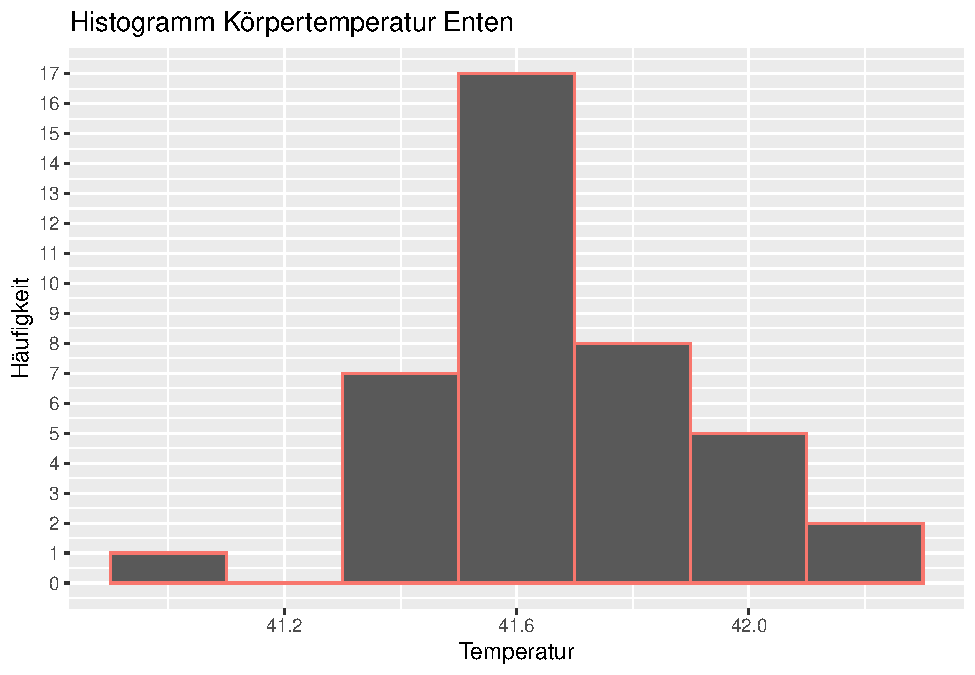
\includegraphics{aps_statistik1_files/figure-latex/unnamed-chunk-6-1.pdf}

Aufgrund dieser Darstellung kann die Veterinärin nun sehen, wie häufig welche Körpertemperature sind. Dies wird die \textbf{Verteilung} des Merkmals genannt. Sie bemerkt zum Beispiel, dass Beobachtungen der Körpertemperatur rund um 41.6°C am häufigsten sind und tiefere und höhere Temperaturen seltener vorkommen. Auf einen Blick sieht sie auch, dass die Temperatur aller Enten zwischen 41°C und 42.2°C war.

Die Verteilung eines Merkmals zu kennen ist hilfreich, jedoch in vielen Situationen (z. B. in der Kommunikation) noch zu komplex. Einfacher ist es die Komplexität einer Verteilung auf zwei Faktoren herunterzubrechen: Die Zentralität und die Variabilität einse Merkmals.

\subsection{Zentralität}\label{zentralituxe4t}

Mit der Zentralität ist ein Wert gemeint, welcher die zentrale Tendenz des Merkmals abbildet. Um die Zentralität zu messen gibt es drei Möglichkeiten:

\begin{itemize}
\tightlist
\item
  Der \textbf{Modus} ist der am häufigsten vorkommende Wert. Im Beispiel ist das der Wert 41.52, welcher 3 mal und damit am häufigsten vorkommt.
\item
  Wenn die Werte des Merkmals aufsteigend sortiert werden und der Wert betrachtet wird, welcher die Beobachtungen in eine tiefere und eine höhere Hälfte teilt, dann wird dieser Wert als \textbf{Median} bezeichnet. Bei einer geraden Anzahl Beobachtungen, wird in der Regel der Durchschnittswert der beiden mittigsten Beobachtungen verwendet. Im Beispiel haben wir 40 Beobachtugen. Der Median entspricht also dem Durchschnittswert zwischen dem 20. und dem 21. der aufsteigend sortierten Werte
  41.07 41.32 41.35 41.43 41.46 41.46 41.48 41.5 41.51 41.52 41.52 41.52 41.53 41.53 41.54 41.58 41.58 41.6 41.62 41.65 41.66 41.67 41.67 41.69 41.7 41.72 41.8 41.81 41.81 41.82 41.82 41.88 41.89 41.92 41.92 41.96 42.01 42.06 42.14 42.18
  , also 41.655.
\item
  Das \textbf{arithmetische Mittel} bezeichnet, was gemeinhin mit Durchschnitt gemeint ist. Wenn wir die erste von insgesamt \(n\) Beobachtung mit \(x_1\) und die letzte Beobachtung mit \(x_n\) bezeichnen, so ist das aritmethische Mittel
  \[\bar{x} = \frac{1}{n}\sum^n_{i=1} x_i\]
  Im Beispiel ist das arithmetische Mittel der Körpertemperaturen 41.6725.

  Exkurs Wie liest man diese Formel?

  TODO.
\end{itemize}

Jedes dieser Masse für die Zentralität hat Vor- und Nachteile und sie werden dementsprechend in unterschiedlichen Situationen eingesetzt, siehe Übungen.

\subsection{Variabilität}\label{variabilituxe4t}

\section{Übungen}\label{uxfcbungen}

\begin{exercise}
\leavevmode

\begin{enumerate}
\def\labelenumi{(\alph{enumi})}
\tightlist
\item
  Versuche selbst ein Histogramm der Daten oben (\emph{Enten\_n40.sav}) mit Jamovi zu erstellen und begründe, weshalb es nicht gleich aussieht wie das Histogramm oben.
\item
  Berechne zusätzlich das arithmetische Mittel und die Standardabweichung des Merkmals.
\end{enumerate}

\end{exercise}

\begin{solution}
\leavevmode

\begin{figure}
  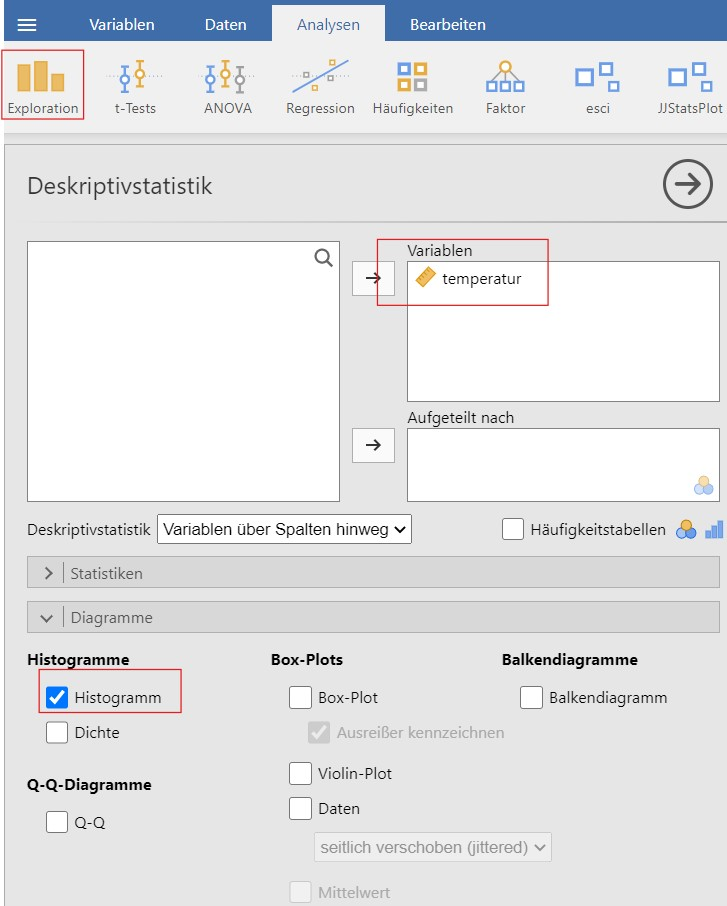
\includegraphics[width=0.5\linewidth]{figures/Enten_n40_instr_histogramm} 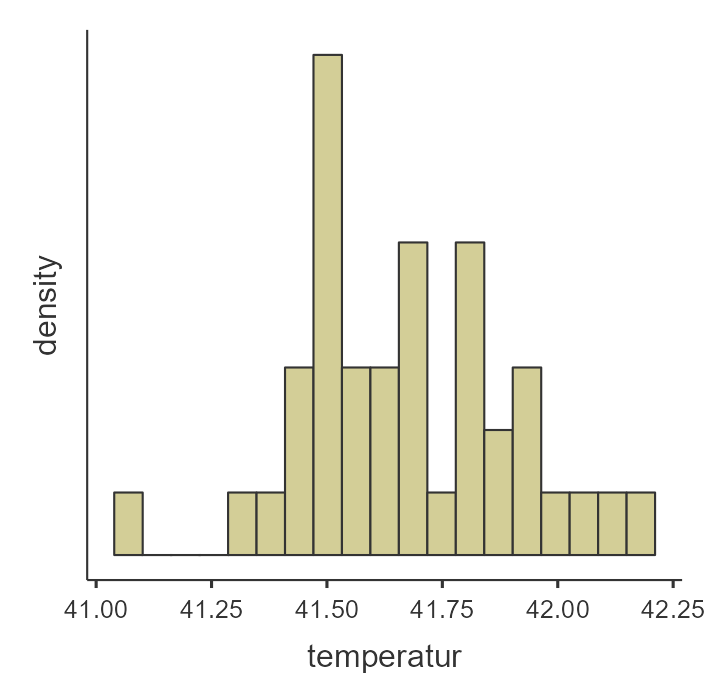
\includegraphics[width=0.5\linewidth]{figures/Enten_n40} \caption{Links: Jamovi-Anleitung zur Erstellung des Histogramms; rechts: Histogramm der Temperatur.}\label{fig:unnamed-chunk-8}
  \end{figure}

\begin{enumerate}
\def\labelenumi{(\alph{enumi})}
\item
  Das Histogramm sieht nicht gleich aus, da Jamovi die Temperaturabschnitte kürzer gewählt hat nämlich bei 0.125°C statt 0.2°C wie oben im Text. In Jamovi gibt es aktuell keine Möglichkeit die Abschnittsweite anzupassen. Ein Histogramm sieht immer anders aus je nach ausgewählter Abschnittsweite.
\item
  TODO
\end{enumerate}

\end{solution}

\begin{exercise}
\leavevmode

\begin{enumerate}
\def\labelenumi{(\alph{enumi})}
\tightlist
\item
  TODO
\item
  TODO
\end{enumerate}

\end{exercise}

\begin{solution}
Text..
\end{solution}

\chapter{Stichprobenziehung}\label{stichprobenziehung}

\section{Was ist das Problem der Stichprobenziehung?}\label{was-ist-das-problem-der-stichprobenziehung}

\section{Wie kann man Aussagen über die Grundgesamtheit machen?}\label{wie-kann-man-aussagen-uxfcber-die-grundgesamtheit-machen}

\section{Übungen}\label{uxfcbungen-1}

\chapter{Durchschnitt und Standardabweichung schätzen}\label{durchschnitt-und-standardabweichung-schuxe4tzen}

\section{Wo liegt der Durchschnitt der Grundgesamtheit?}\label{wo-liegt-der-durchschnitt-der-grundgesamtheit}

\section{Wo liegt der Durchschnitt der Standardabweichung?}\label{wo-liegt-der-durchschnitt-der-standardabweichung}

\section{Übungen}\label{uxfcbungen-2}

\chapter{Durchschnitt testen}\label{durchschnitt-testen}

\section{Entspricht der Durchschnitt der Grundgesamtheit einem gewissen Wert?}\label{entspricht-der-durchschnitt-der-grundgesamtheit-einem-gewissen-wert}

\section{Weicht der gefundene Durchschnitt stark vom hypothetischen Wert ab?}\label{weicht-der-gefundene-durchschnitt-stark-vom-hypothetischen-wert-ab}

\section{Übungen}\label{uxfcbungen-3}

\part{Gruppenvergleich einer intervallskalierten Variable}\label{part-gruppenvergleich-einer-intervallskalierten-variable}

\chapter{Gruppenvergleich einer intervallskalierten Variable}\label{gruppenvergleich-einer-intervallskalierten-variable}

\section{Zwei Gruppen vergleichen}\label{zwei-gruppen-vergleichen}

\section{Was ist das Problem der Stichprobenziehung?}\label{was-ist-das-problem-der-stichprobenziehung-1}

\section{Wie kann man Aussagen über die Grundgesamtheit machen?}\label{wie-kann-man-aussagen-uxfcber-die-grundgesamtheit-machen-1}

\section{Übungen}\label{uxfcbungen-4}

\chapter{Welch-Test}\label{welch-test}

\section{Zwei Gruppen vergleichen}\label{zwei-gruppen-vergleichen-1}

\section{Sind die Durchschnitte der beiden Gruppen in der Grundgesamtheit gleich?}\label{sind-die-durchschnitte-der-beiden-gruppen-in-der-grundgesamtheit-gleich}

\section{Wie stark unterscheiden sich die Durchschnitte?}\label{wie-stark-unterscheiden-sich-die-durchschnitte}

\section{Übungen}\label{uxfcbungen-5}

  \bibliography{book.bib,packages.bib}

\end{document}
